\problemname{Australian Open}


\begin{figure}[!h]
\begin{center}
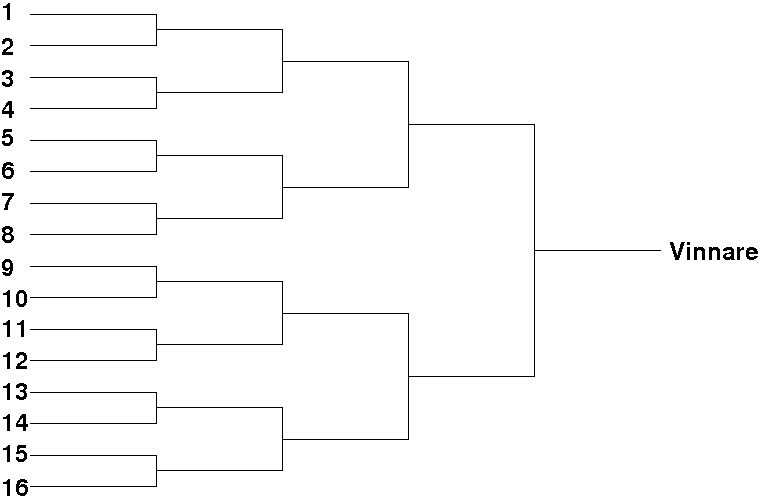
\includegraphics[width=0.5\textwidth]{australian.png}
\end{center}
\end{figure}

This year's big sports event in Australia is of course the International Olympiad in Informatics. While waiting for this, some side events have been organized, for example the tennis tournament Australian Open. This is an \emph{elimination tournament} that can
be described with a bracket according to the figure above, where the number of \emph{rounds} $n$ can vary. One starts on the left with $2^n$ players, numbered from 1 to $2^n$. After a total of $2^n - 1$ matches, a winner is determined.

We now assume that each player $i$ has an ``ability'' $x_i$, and that when two players $i$ and $j$ meet, player $i$ wins with probability
\begin{displaymath}
P(i \text{ defeats } j) = \frac{1}{1+\exp(x_j-x_i)}
\end{displaymath}
and otherwise player $j$ wins since a tennis match cannot end in a
draw ($\exp(x)$ denotes the exponential function $e^x$). The formula is chosen so that $P(i \text{ defeats } j)+P(j \text{ defeats } i)=1$.

Write a program that, given all players' abilities, determines who has
the greatest chance of winning the tournament and how large that chance is.


\section*{Input}
The first line contains an integer $n$ ($1 \leq n \leq 10$), the number of rounds.
The second line contains $2^n$ floating-point numbers between 0 and 10, the ability of
each player in numerical order.

\section*{Output}
Output an integer and a floating-point number: the number of the player who has
the greatest chance of winning the tournament and the probability that this player
wins. If several players have the greatest chance, you may output any
of them. The answer is accepted if the absolute error is less than $10^{-5}$.

\section*{Scoring}
Your solution will be tested on a set of test groups.
To earn points for a group, you must pass all test cases in that group.

\noindent
\begin{tabular}{| l | l | p{12cm} |}
  \hline
  \textbf{Group} & \textbf{Points} & \textbf{Constraints} \\ \hline
  $1$    & $20$       & $n=1$ \\ \hline
  $2$    & $80$       & No additional constraints. \\ \hline
\end{tabular}

\section*{Explanation of Sample 1}
The first match is won by player 1 with probability 0.549834 and by player 2 with probability 0.450166.
The second match is won by player 3 with probability 0.689974 and by player 4 with probability 0.310026.
These events are independent and thus we can compute the probability
for each possible final pairing by multiplying the probabilities with
each other. This gives rise to the following table:

\begin{tabular}{|c|c|c|c|c|c|c|} \hline
 & {\bf Probability of} & {\bf Probability of} & \multicolumn{4}{|c|}{\bf Contribution to total chance player wins}  \\
{\bf Match} & {\bf match being played} & {\bf winning the match} & {\bf
  1}&{\bf 2}&{\bf 3}&{\bf 4} \\ \hline
1--3 & 0.379371 & 0.524979--0.475021 & 0.199162 & -- & 0.180209 & -- \\
1--4 & 0.170463 & 0.710950--0.289050 & 0.121190 & -- & -- & 0.049272 \\
2--3 & 0.310603 & 0.475021--0.524979 & -- & 0.147543 & 0.163060 & -- \\
2--4 & 0.139563 & 0.668188--0.331812 & -- & 0.093254 & -- & 0.046309 \\ \hline
{\bf Sum }& {\bf 1.000000} &                & {\bf 0.320352} & {\bf 0.240797} & {\bf 0.343269 }& {\bf 0.095581 } \\ \hline
\end{tabular}
